\documentclass{scrartcl}
%% $Id: multi-after1s1c.tex 112 2021-06-14 08:01:42Z herbert $

\documentclass[a4paper,11pt]{article}
\usepackage[color]{lapdf}
\textheight25.12cm
\textwidth18.92cm
\oddsidemargin-1.5cm
\evensidemargin-1.5cm
\topmargin-0.5cm
\topskip0cm
\headheight0cm
\headsep0cm
\parskip0.5cm
\parindent0cm
\unitlength1cm



\begin{document}
\title{Example for fullpage floats}
\author{Herbert Voß}
\maketitle

\tableofcontents

\blinddocument

\section{File \texttt{\jobname}}

\begin{lstlisting}
The multi images~\vref{img:demo0} has a caption~\vpageref{img:demo0-cap}.
\end{lstlisting}

The fullpage multifloat~\vref{img:demo0} has a caption~\vpageref{img:demo0-cap}.


\begin{lstlisting}
\captionsetup{singlelinecheck=false}
\hvFloat[fullpage,capPos=after,multiFloat,vFill]%
  +{figure}{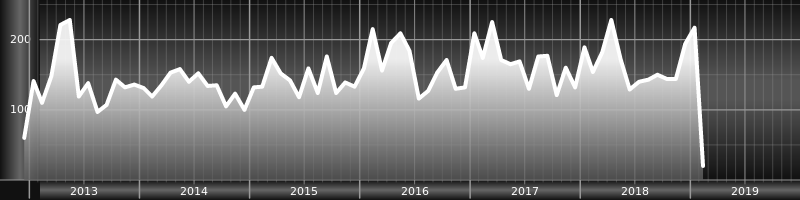
\includegraphics[width=\linewidth]{CTAN}}%%                   no 1
   [Short caption A]%
   {A Caption A of a ``fullpage'' object, which follows on the left or
    right column. This can be an even or odd page. And some more text whch has no
    real meaning because it fills only the space for a long caption.}%
   {img:demo0}%
  +{table}{\begin{tabular}{lrcp{3cm}}\hline                 %             no 2
            Linksbündig & Rechtsbündig & Zentriert & Parbox\\\hline
            L           & R            & C         & P\\
            left        & right        & center    & Text with possible linebreaks\\
            \multicolumn{4}{c}{Multicolumn over all columns}\\\hline
           \end{tabular}}%
   [Short Caption B]%
   {A Caption B of a ``fullpage'' object, which follows on the left or
        right column. This can be an even or odd page.}{}%
  +{figure}{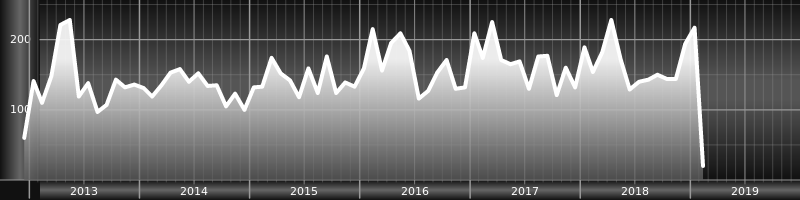
\includegraphics[width=\linewidth]{CTAN}}%%                    no 3
   {A Caption C of a ``fullpage'' object, which follows on the left or
      right column.}%
   {img:demo1}
  +{figure}{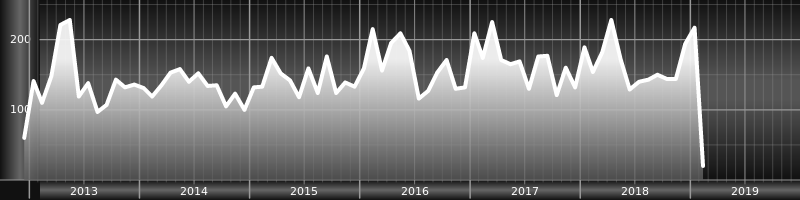
\includegraphics[width=\linewidth]{CTAN}}%%                    no 4
   {A Caption C of a ``fullpage'' object, which follows on the left or
      right column.}%
   {img:demo2}
\end{lstlisting}


\Float[Multi]
\captionsetup{singlelinecheck=false}
\hvFloat[fullpage,capPos=after,multiFloat,vFill]%
  +{figure}{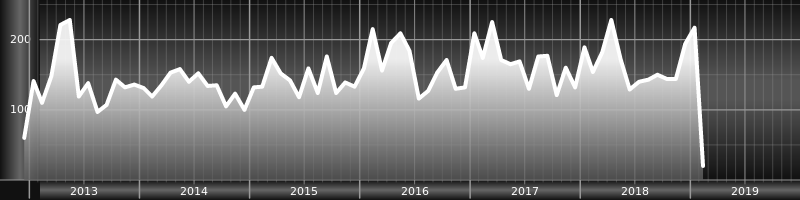
\includegraphics[width=\linewidth]{CTAN}}%%  no 1
   [Short caption A]%
   {A Caption A of a ``fullpage'' object, which follows on the left or
    right column. This can be an even or odd page. And some more text whch has no
    real meaning because it fills only the space for a long caption.}%
   {img:demo0}%
  +{table}{\begin{tabular}{lrcp{3cm}}\hline                 %             no 2
            Linksbündig & Rechtsbündig & Zentriert & Parbox\\\hline
            L           & R            & C         & P\\
            left        & right        & center    & Text with possible linebreaks\\
            \multicolumn{4}{c}{Multicolumn over all columns}\\\hline
           \end{tabular}}%
   [Short Caption B]%
   {A Caption B of a ``fullpage'' object, which follows on the left or
        right column. This can be an even or odd page.}{}%
  +{figure}{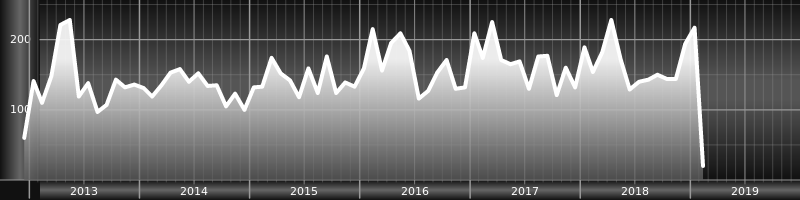
\includegraphics[width=\linewidth]{CTAN}}%%  no 3
   {A Caption C of a ``fullpage'' object, which follows on the left or
      right column.}%
   {img:demo1}
  +{figure}{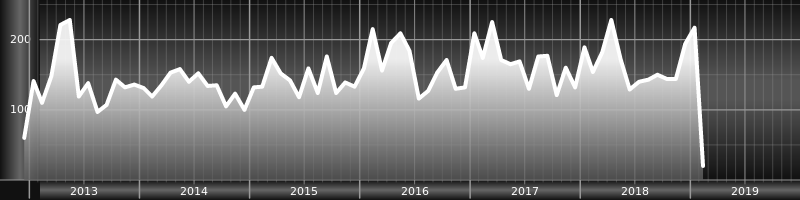
\includegraphics[width=\linewidth]{CTAN}}%%  no 4
   {A Caption D of a ``fullpage'' object, which follows on the left or
      right column.}%
   {img:demo2}



\Blindtext


\begin{lstlisting}
\captionsetup{singlelinecheck=false}
\hvFloat[fullpage,capPos=after,multiFloat,vFill]%
  +{figure}{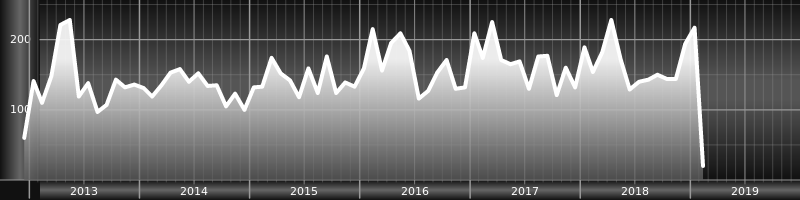
\includegraphics[width=\linewidth]{CTAN}}%%                   no 1
   [Short caption A]%
   {A Caption A of a ``fullpage'' object, which follows on the left or
    right column. This can be an even or odd page. And some more text whch has no
    real meaning because it fills only the space for a long caption.}%
   {img:demo3}%
  +{table}{\begin{tabular}{lrcp{3cm}}\hline                 %             no 2
            Linksbündig & Rechtsbündig & Zentriert & Parbox\\\hline
            L           & R            & C         & P\\
            left        & right        & center    & Text with possible linebreaks\\
            \multicolumn{4}{c}{Multicolumn over all columns}\\\hline
           \end{tabular}}%
   [Short Caption B]%
   {A Caption B of a ``fullpage'' object, which follows on the left or
        right column. This can be an even or odd page.}{}%
  +{figure}{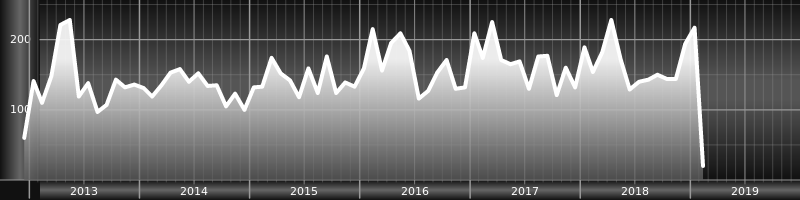
\includegraphics[width=\linewidth]{CTAN}}%%                    no 3
   {A Caption C of a ``fullpage'' object, which follows on the left or
      right column.}%
   {img:demo4}
  +{figure}{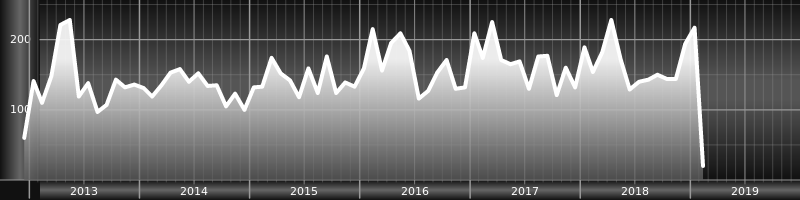
\includegraphics[width=\linewidth]{CTAN}}%%                    no 4
   {A Caption C of a ``fullpage'' object, which follows on the left or
      right column.}%
   {img:demo5}
\end{lstlisting}

\Float[Multi]
\captionsetup{singlelinecheck=false}
\hvFloat[fullpage,capPos=after,multiFloat,vFill]%
  +{figure}{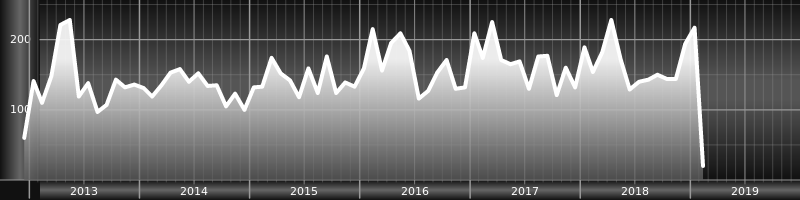
\includegraphics[width=\linewidth]{CTAN}}%%  no 1
   [Short caption A]%
   {A Caption A of a ``fullpage'' object, which follows on the left or
    right column. This can be an even or odd page. And some more text whch has no
    real meaning because it fills only the space for a long caption.}%
   {img:demo3}%
  +{table}{\begin{tabular}{lrcp{3cm}}\hline                 %             no 2
            Linksbündig & Rechtsbündig & Zentriert & Parbox\\\hline
            L           & R            & C         & P\\
            left        & right        & center    & Text with possible linebreaks\\
            \multicolumn{4}{c}{Multicolumn over all columns}\\\hline
           \end{tabular}}%
   [Short Caption B]%
   {A Caption B of a ``fullpage'' object, which follows on the left or
        right column. This can be an even or odd page.}{}%
  +{figure}{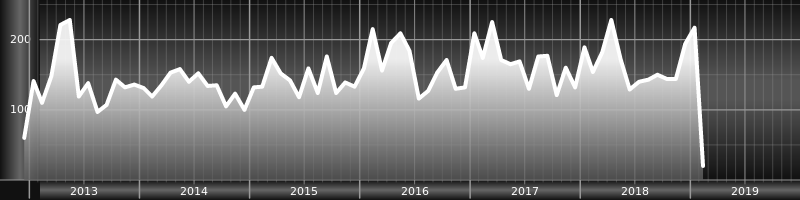
\includegraphics[width=\linewidth]{CTAN}}%%  no 3
   {A Caption C of a ``fullpage'' object, which follows on the left or
      right column.}%
   {img:demo4}
  +{figure}{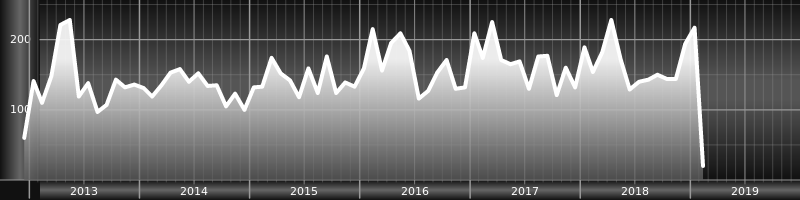
\includegraphics[width=\linewidth]{CTAN}}%%  no 4
   {A Caption D of a ``fullpage'' object, which follows on the left or
      right column.}%
   {img:demo5}


\blinddocument

\Blindtext

\blindtext


\end{document}